\section{Snell波与斜坐标}
\label{sec:5.3}

倾斜叠加与Snell波紧密有关,但事情还不仅止于此,三种不同类型的道集(共炮点道
集,共检波点道集及共中心点道集)都可以作倾斜叠加,而在每种情形下其意义却均不相
同。

一个Snell波可以用普通反射数据进行倾斜叠加的办法把它合成出来,凡Snell波都可按
波动传播理论加以描述,尽管有横向速度变动、多次反射、横波等复杂性或者所有这些复杂
情形同时存在,你仍可望能够写出一个真实描述Snell波的波动方程。与此形成对照的是
CDP叠加,在这里,向下延拓就已经是一种近似了,即使在速度为常数时也是如此。我们当
然总可以返回炮点检波点空间内去作数据分析,但倾斜叠加是一种叠加处理,因而那就意味
着已经作过干扰处理和数据压缩了。

\subsection{野外资料中的Snell波信息}
\label{sec:5.3.1}

根据叠加原理,我们能由具有一切频率之正弦波的叠加形成一个脉冲函数,推广至三维
情形,沿所有方向传播之平面波叠加起来则形成一个点震源。与此相似,一个平面波可以是由
许多惠更斯二次点源叠加所成的结果,对勘探中所记录的点震源数据采取一种称为倾斜叠加
的适当叠加处理,则可以模拟Snell波。

假想一条地震测线内的所有炮点都在同一时间起爆,这时的下行波将近似为平面波(假
设我们忽略真实世界是三维而不是二维这个现实),由这样一种排列所记录到的资料完全可
以根谄常规资料模拟出来,只须将数据场遍及所有炮点坐标s求和即可\footnote{
设野外记录为户$(s, g,t)$,
其中,s为炮点坐标,g为检波点坐标,t为时间。取共检波点道集$p(s_1, g,
t)$, $p(s_2,g,t)$,......,不经动校正而全部直接叠加、因反射波时距曲线在检波点g附近的曲率较平缓,故为同相叠加而加
强,远离该点则因非同相干涉而减弱,因此得出$(g,t)$
空间内的近似上行平面波。如取共炮点道集$p(s, g_1, t)$、$p(s,
g_2,t)$,......作相同叠加处理,则得$(s,t)$空间内的近似下行平面波。---译者
},每个共
检波点道集内的各记录道要不经正常时差校正就求和。

要想模拟某种非垂直方向传播的Snell波,则必须按照所需描述的某个射线参量值$p_s=
dt/ds$使相继的激发保持一定的时间延迟,犹如是从水平飞行的超音速飞机所辐射出来的一
般。

如果是沿检波点坐标轴g而不是沿炮点坐标轴s将数据求和,情形会如何?这时所得结果
相当于业已准确调谐至只接收垂向传播之波的接收天线所记录的点源试验\footnote{
这段的意思是说:共炮点道集不经正常时差校正而直接叠加求和所得相当于炮点坐标空间$(s,t)$内的自激自收下行平面波。 ---译者
},在叠加求和之
前使检波点上的到达时间有时移,则可模拟只记录某一种Snell波的接收天线,比方说,记录
到参量为$p_g=dt/dg$、上行角度为$\sin\theta=p_gv$的波。

沿某一坐标轴进行积分就是沿某一坐标轴进行低通滤波的一种极端情形,介于点震源情
形和平面波情形这两种极端之间的是定向发射与接收的情形。

简单的传播过程使点源扰动散布至一定距离之处,波就似乎是有些像平面波或Snell波
了,这样就可以把波至显得几乎是呈平面形状之处的一小段同相轴当作Snell波进行分析。

总而言之,在炮点空间$(s,t)$内进行倾角滤波所得到的是下行Snell波,而在检波点
空间$(g,t)$内进行倾角滤波所得到的则是上行Snell波。


\subsection{噪音抑制与数据记录}
\label{sec:5.3.2}

噪音抑制(muting)的基本目的是消除水平传播的能量\footnote{
muting是常规地震处理中的一科预处理程序,又可译为切除处理,目的在于切除直达波和面波干扰,即所谓的水
平传播的能量。---译者
},这类能量与地层映象毫无关
系。典型的实现抑制切除之方法如\ref{sec:3.5}节所述,那就是说,采用某种加权函数将普遍超出炮
检距与时间之比值$(g-s)/t$某个门限值的数据均置零。噪音抑制处理可以切除许多水平传播
能量是没疑问的,但是要消除的还不仅限于此。因反向散射之故,常常在噪音抑制区之内还可
发现水平传播的能量,除掉它的办法必须采用倾角滤波而不是采用某种加权函数。在现代高
密度多道记录系统采用以前,低速传播的噪音往往在检波器电缆长度范围内形成空间假频现
象,以致进行倾角滤波行不通.如果出射角并非足够接近于垂直,就是说,如果$dt/dg$不是
足够小,这时波就可能不是来自勘探目的层。在炮点空间$(s,t)$内应用滤波不像在检波点
空间$(g,t)$内那么容易,因为在炮点空间内极少能非常稠密地记录数据。千万别跌入圈
套,认为可以对共中心点道集进行这种倾角滤波,反向散射的地滚波在共中心点道集内是没
有正常时差的(见\ref{sec:3.2}节)!

海水层底部散射往往很强,使得很难采用常规处理方法压制它。在\ref{sec:3.2}节中,我们已了
解其原因在于点溫散射意味着有双曲线型波至,它具有陡倾角,其到达时间一般比水层底部
反射时间要晚,因而会误认为它们具有沉积地层的叠加速度而不是水层速度。这时所需要的
是作两种倾角滤波,一种是抑制以非垂直角度离开各炮点的波,另一种则是抑制以非垂直角
度到达各检波点的波。现今的野外组合其滤波作用系以空间频率$k_x$为基础,如记录设备采用倾
角$(k/\omega)$的滤波而不是采用空间频率的滤波,资料中将会留有更多高频能量。\ref{sec:2.5}节中所
述具有时间因果性的递归倾角滤波在这里可能会起很好的作用。


\subsection{Snell波的合成}
\label{sec:5.3.3}

设我们用野外数据人工合成了一个下行的Snell波,然后设想一下上行波将会显得如何,
以及它将如何把有关地下界面的信息带给我们。

进行倾斜叠加要取测线上的数据$P(s,g,t)$,它是炮点位置s、检波器位置g和旅行时
间t的一个函数。然后,要在炮点遍及的范围内求和,从而合成作出犹如应当是由下行Snell波
发生了反射才能被记录到的上行波$U(g,t)$。即使可能存在有速度横向变化和多次反射,
情形仍应如此,不受影响。

因为涉及到三种不同类型的时间,求和过程有点混乱:
t=点震源野外记录内的时间。\\
$t'=t-p(g-s)$=解释时间。仅在$t'=0$之后才看得见最浅的反射面。\\
$t_{pseudo}$=具有移动震源之Snell假想排列记录内的时间。\\

在水平成层地层情形下,假想排列记录内的时间$t_{pseudo}$具有特定的特征:你将检波点坐标
移出越远,回声反射就会到达越晚。根据下列关系可从野外排列记录的时间t直接变换为解释时间t':
\begin{equation}
t'=t_{pseudo}-px=t-p(g-s)
\label{eq:ex5.3.1}
\end{equation}
图\ref{fig:slnt/snellwave}示意绘出了下行Snell波的情形。

\begin{figure}[H]
\centering
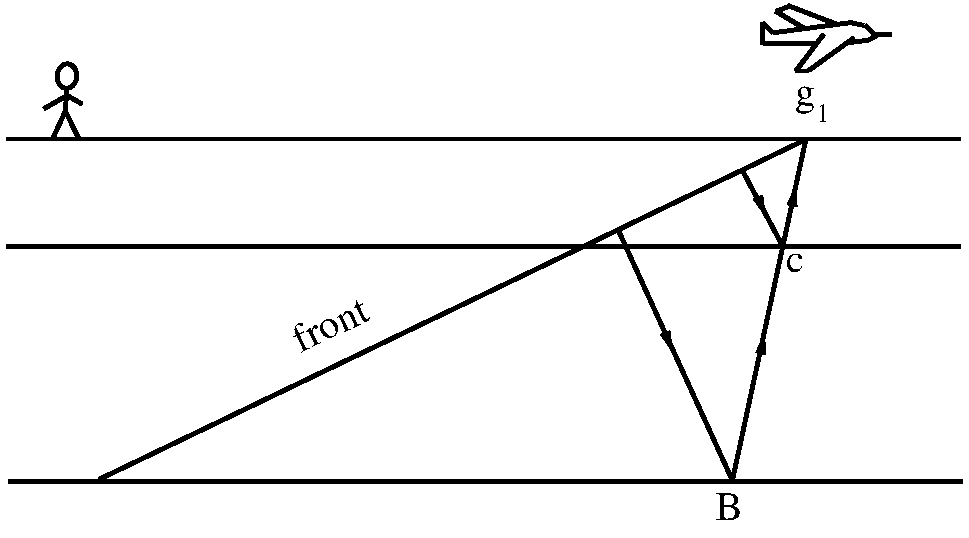
\includegraphics[width=0.65\textwidth]{slnt/snellwave}
\caption[snellwave]{Snell波的波阵面由两个地层反射,携带信息
上行返回至检波器$g_1$
}
\label{fig:slnt/snellwave}
\end{figure}

图\ref{fig:slnt/cspss}所示是一种假设的共检
波点道集,将该道集求和可模拟出图
\ref{fig:slnt/snellwave}中所见到的位于$g_1$上之Snell波。在图\ref{fig:slnt/snellwave}
中的由C点至B点的横向偏离距离与图\ref{fig:slnt/cspss}中相应的距离(图\ref{fig:slnt/cspss}中的两
个位置上)是完全相等的。对所有的检波点
重复进行上述沿炮点坐标的求和过程,即可由下行Snell波作出合成上行波。

\begin{figure}[H]
\centering
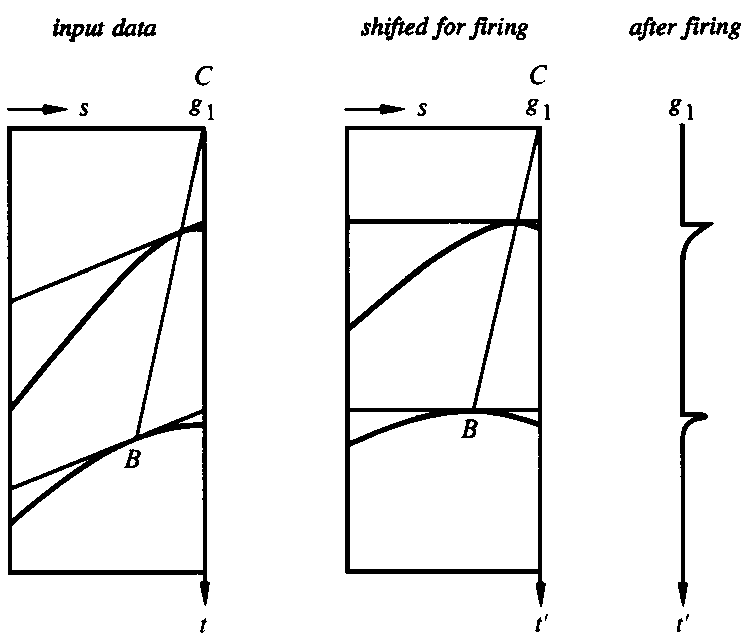
\includegraphics[width=0.65\textwidth]{slnt/cspss}
\caption[cspss]{左图是两个平反射界面情形下的位于
检波点$g_1$上的共检波点道集。中图表示,为准备用遍及炮点
坐标s进行求和而产生合成Snell波,数据已根据线性时差校正作
了时移。右图所示是检波点$g_1$上所记录到的Snell波记录道。
Snell波的地震剖面由许多像$g_1$的记录道并列组成。
}
\label{fig:slnt/cspss}
\end{figure}

因为仅在$t'=0$之后才看见找层反射面,而且水平地层的回声反射不同于
假想的Snell波,其到达并不具有水平方向
时差,所以可将变量$t'$称作是解释坐标。在水平地层情形下,对横向位置进行检测
得依靠反射系数的横向变化。在图\ref{fig:slnt/snellwave}
中,关于B点的反射强度之信息是在右侧
的$g_1$点上记录到的,不是像常规叠加那样在B点的正上方之处才能见到它。为了得到完美解
释结果,因而得额外要求把所接收数据移动到一个适当的横向位置上去。

图\ref{fig:slnt/interpcoord}所示是与图\ref{fig:slnt/snellwave}和\ref{fig:slnt/cspss}相同之两个平界面,但在A、B和C各点上还有异常的反射系数,A点位于B点正上方,
由B点所反射的波其路程直接通
过C点,再从C点到达检波点$g_1$。 
相继各个画面所示均为与这三个
点有关的绕射双曲线。注意,从
两个平界面发生反射的假想
Snell波其时差变化率均为办由 
散射点B与C形成的双曲线
与各该Snell波分别在a、b与c各 
点上相切;注意b与c位于仍点正
下方的情形,是因为它们全都沿 
Snell参量为p的一个射线路程排
列成行而形成的。由于不论入射 
波场情形如何,最早到达的波至
必然应位于散射点之正上方,所 
以右上图中的A、B和C各点均应
位于各该双曲线的顶部。转换为 
左下图中的解释坐标t'时,能得
到的主要好处是来自水平地层的 
波至都变成水平的了。但是要注
意,各该双曲面业已变得偏斜。
当把我们的注意力局限于具有微
小时差的那一部分波至时,我们
可以发现关于异常反射系数的信
息全部都位于a、b和c各点邻域
内,而这些点原来都是处于双曲线的侧翼上的。不把相应数据向左侧横向移动,比方说,
移至$g'=g-f(t')$,这些点是不会占有正确几何位置的,亦即不会占据原有的A、B和C点的
位置;作过横向移动后,a点将位于b点之上。正确的移动量大小$f(t')$是一个涉及到速度分析
的问题,从属这种问题的速度分析将在下节讨论。

\begin{figure}[H]
\centering
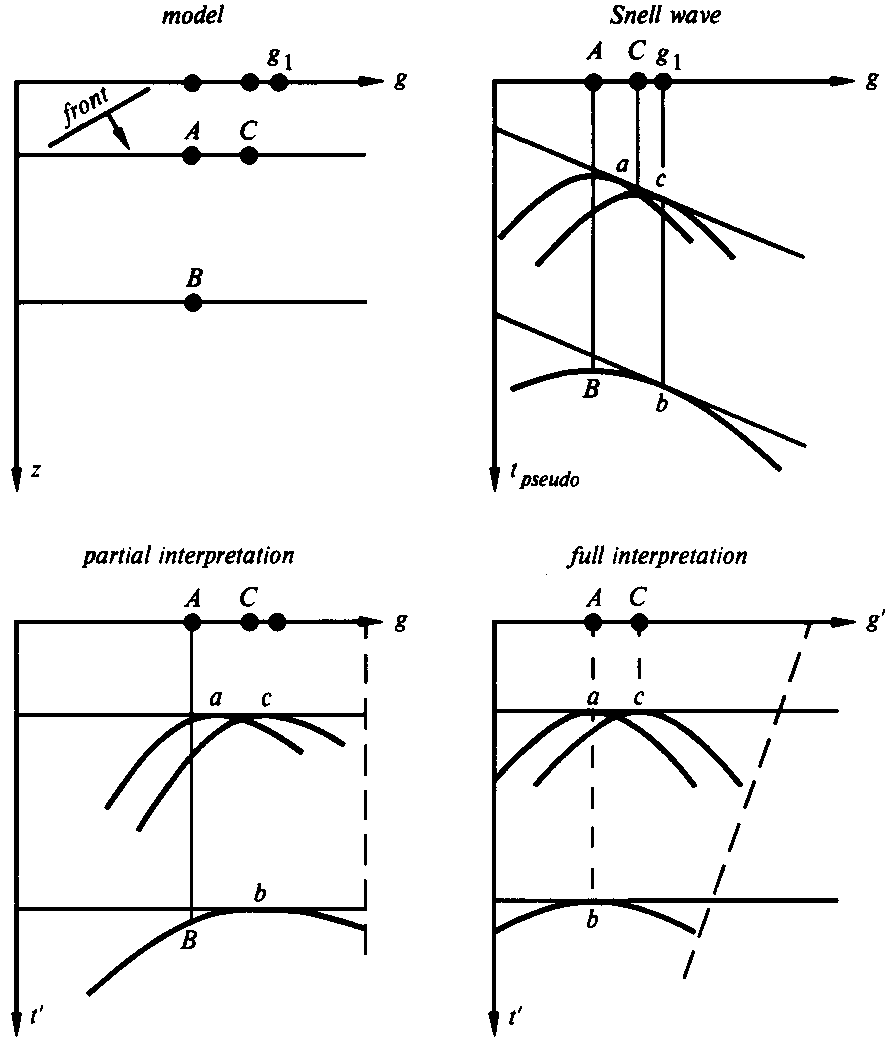
\includegraphics[width=0.65\textwidth]{slnt/interpcoord}
\caption[interpcoord]{左上图为两个反射面上的三个点散射体义A,B,C。右上图
为所期望之Snell波。左下图为经过线性时差校正之后的Snell波。
右下图为转换至完整的解释坐标之后的情形,在最后的这个结果
中a,b与c各点均已位于幵始时的A、B与C各点位置上了
}
\label{fig:slnt/interpcoord}
\end{figure}

\subsection{Snell波出了啥毛病?}
\label{sec:5.3.4}

在建立平方根方程以前,我曾经认为进行地震数据分析的唯一正确途径就是把它分解成
Snell波。既然一个Fresnel带看来不过就大约10°左右,要不了多少Snell波也就行了。只需
少量剖面曾经是很重要的。因为七十年代的计算机能力很有限。当时我知道藉助于一个平方
根方程每个Snell波都是可分析的,而且知道即使是多次反射也可以采用《地球物理数据处
理基础》一书中和本书\ref{sec:5.6}节中所述方法来加以处理。从理论上说,这种办法可算得上是对完
全难以分析的CDP叠加所作过的一项重大改进了
。然而,对于下行Snell波来说,存在有一个
实际问题,这就是:当它们离开地表面之后不久就遇到横向速度不均匀性,它们也许早就
变得很复杂了。虽然我对它们将会有什么最终作用还不能肯定,我是不再相信Snell波是一
种包治百病的灵丹妙药了。但是,许多波都表现出它们有一点儿像是Snell波,这一点触动
了我要去建立发展一种对Snell波来说是理想的坐标系统,而对有一点像是Snell波的那些波
来说则是有效的坐标系统。

\subsection{横向不变性}
\label{sec:5.3.5}

垂直入射力$p=0$平面波震源在水平层状介质内产生的反射波场具有横向不变性,换言
之,有关波场的观测与理论在这种情形下所具有的形式均属$P(t)\times const(x)$。在任何特定的
非零值情形下的Snell波也都是横向不变的,就是说,利用新坐标
\begin{subequations}
\begin{equation}
t'=t-px
\label{eq:ex5.3.2a}
\end{equation}
\begin{equation}
x'=x
\label{eq:ex5.3.2b}
\end{equation}
\label{eq:ex5.3.2}
\end{subequations}
则横向不变性可由下述陈述给出
\begin{equation}
P(x,t)=P'(t')\times const(x')
\label{eq:ex5.3.3}
\end{equation}
显然,当一个貌似二维的问题可以简化成一维问题时,会产生重大概念上的好处,更不用说
采样和计算上的好处了。在继续进行讨论之前,要研究一下方程\ref{eq:ex5.3.3}直到你确实理解
了当如条件\ref{eq:ex5.3.2b}所述$x'=x$时,为什么波场可以随x而变化但却是x'的一种常值函数。


坐标系统\ref{eq:ex5.3.2}是延迟坐标系统,不是一种运动坐标系统。在固体地球物理学中,
采用运动坐标系统进行计算是很糟糕的,地层内的速度函数从来不是时变的(time-variable),可是在运动坐标系统内它却成为时变的了,这会增加计算的复杂性。我们的目标是采用
某一模型速度由数据形成影像,该速度是所有空间维次的一项函数。但是所利用的坐标系统
将具有这么一种参考速度,它仅仅是深度之函数。

\subsection{Snell波的坐标系统}
\label{sec:5.3.6}

Snell波有三个固有平面,受此启发,可用它们构成一坐标系统,第一个平面是恒定深
度z处的地层平面,其中包括地表面。第二个是射线平面。第三个是运动着的波阵面平面,
当速度随深度而变化时,该平面变成曲面。

下列方程定义了Snell波坐标系统
\begin{subequations}
\begin{equation}
z'(z,x,t)=z\frac{\cos\theta}{v}
\label{eq:ex5.3.4a}
\end{equation}
\begin{equation}
x'(z,x,t)=z\tan\theta+x
\label{eq:ex5.3.4b}
\end{equation}
\begin{equation}
t'(z,x,t)=z\frac{\cos\theta}{v}-x\frac{\sin\theta}{v}+t
\label{eq:ex5.3.4c}
\end{equation}
\label{eq:ex5.3.4}
\end{subequations}

方程\ref{eq:ex5.3.4a}利用钻孔中见到的垂直相速度直接定义了旅行时间深度,地层内部的分
界面都正好是恒定z'值处的平面。

令方程\ref{eq:ex5.3.4b}所定义的x'等于常数,比如说,等于$x_0$,则得出射线方程,即
$(x-x_0)/z=-\tan\theta$,不同的$x_0$值代表不同的射线。

令方程\ref{eq:ex5.3.4c}所定义的t'等于常数,则给出运动着的波阵面之方程。要看出这点
令$t'=t_0$并注意在恒定x值时,你看到的是钻井中的速度,而在恒定z值时,你看到的是飞机
的速度。

从数学上说,具有三个未知数的一个方程定义了一个平面,所以,令式\ref{eq:ex5.3.4}中任
何一个方程的左端为常数,就得出在空间内定义了一个平面的方程。为进行实际检验,
不妨考虑一下两个平面相交的情形。使波阵面停留不动得要求$dt'=0$,利用方程\ref{eq:ex5.3.4c},得出
\begin{equation}
dt'=0=\frac{\cos\theta}{v}dz-\frac{\sin\theta}{v}dx+dt
\label{eq:ex5.3.5}
\end{equation}
将该恒定波阵面方程$dt'=0$同恒定深度方程$dz'=dz=0$结合起来,得出了熟悉的关系式
\begin{equation}
\frac{dt}{dx}=p
\label{eq:ex5.3.6}
\end{equation}

在坐标平面是非正交平面时,就说该坐标系统是仿射坐标系统(affine coordinate
system)。利用像\ref{eq:ex5.3.4}那样的仿射坐标,我们无疑易于控制计算,但是我们往往确实也得
遇上给我们自己造成混乱的问题,例如,当我们显示海上野外资料的活动画面时,我们看到
的是一系列共炮点道集$(h,t)$平面;相继的平面就是相继的炮点,所以当我们打算在正交
坐标$(y,h)$或$(s,g)$中考虑问题时\footnote{
y为中心点坐标,h为半炮检鉅,g为检波点坐标,s为炮点坐标。 ---译者
},数据是显示在$(s,h)$平面中的。采用仿射坐
标时,我发现最容易忘掉坐标轴而考虑用垂直的平面来代替。炮点坐标轴s可以被当作是一
个共检波点平面来考虑,比如说,当作是$cg$。所以,我把海上勘探数据活动电影当作是存在于
$(cs,ch,ct)$空间中。在这个活动电影中,另一个平面,实际上是一个平面族、即共中心
点平面cy,随同数据的“分层结构”(见\ref{sec:3.0}节)而一起扫描通过屏幕。

要在速度随深度而变化时定义Snell坐标,仅需要仔细地解释方程\ref{eq:ex5.3.4}。首先,所有
的角度必须利用Snell置换$Sin\theta=pv(z)$通过p来表示,然后z必须赴处用对z的积分来代替。


\subsection{Fourier空间中的Snell波}
\label{sec:5.3.7}

根据偏微分方程连锁法(chain rule),应有
\begin{equation}
\begin{pmatrix}
\partial_t \\
\partial_x \\
\partial_z 
\end{pmatrix}
=\begin{pmatrix}
t_t' & x_t' & z_t'\\
t_x' & x_x' & z_x'\\
t_z' & x_z' & z_z'
\end{pmatrix}
=
\begin{pmatrix}
\partial_{t'} \\
\partial_{x'} \\
\partial_{z'} 
\end{pmatrix}
\label{eq:ex5.3.7}
\end{equation}

在Fourier空间内,上述方程中涉及时间t与水平坐标x的部分可解释为
\begin{subequations}
\begin{equation}
-i\omega=-i\omega'
\label{eq:ex5.3.8a}
\end{equation}
\begin{equation}
ik_x=+p\omega'+ik_x'
\label{eq:ex5.3.8b}
\end{equation}
\label{eq:ex5.3.8}
\end{subequations}
在线性时差校正(对x'保持恒定)之后变得平缓的同相轴能量具有特殊意义,对于这类能量应
有$\partial/\partial x'=ik_x'=0$,于是将式\ref{eq:ex5.3.8a}与
\ref{eq:ex5.3.8b}结合起来可得出熟悉的关系方程
\begin{equation}
p=\frac{k}{\omega}
\label{eq:ex5.3.9}
\end{equation}

\subsection{习题}
\label{sec:5.3.8}
\begin{enumerate}
\item 试解释图\ref{fig:slnt/cspss}中的s坐标轴应如何选取符号。
\item 方程\ref{eq:ex5.3.4}属于上行Snell波的情形,试问:适用于下行Sneir波的将是何种坐
标系统。
\item 试在坐标系统\ref{eq:ex5.3.4}内表示标量波动方程。忽略其一阶导数项。
\item 试按照Fourier变量$(\omega ',k_z',k_x')$来表7K标量波动方程的波散关系。
\end{enumerate}












